\documentclass{standalone}
\usepackage{tikz}
\usetikzlibrary{patterns}
\usetikzlibrary{positioning}
\usetikzlibrary{patterns, positioning}
\usetikzlibrary{shapes.misc}
\usepackage[outline]{contour}
\contourlength{1.5pt} 
\usepackage[sfdefault]{ClearSans}

\begin{document}
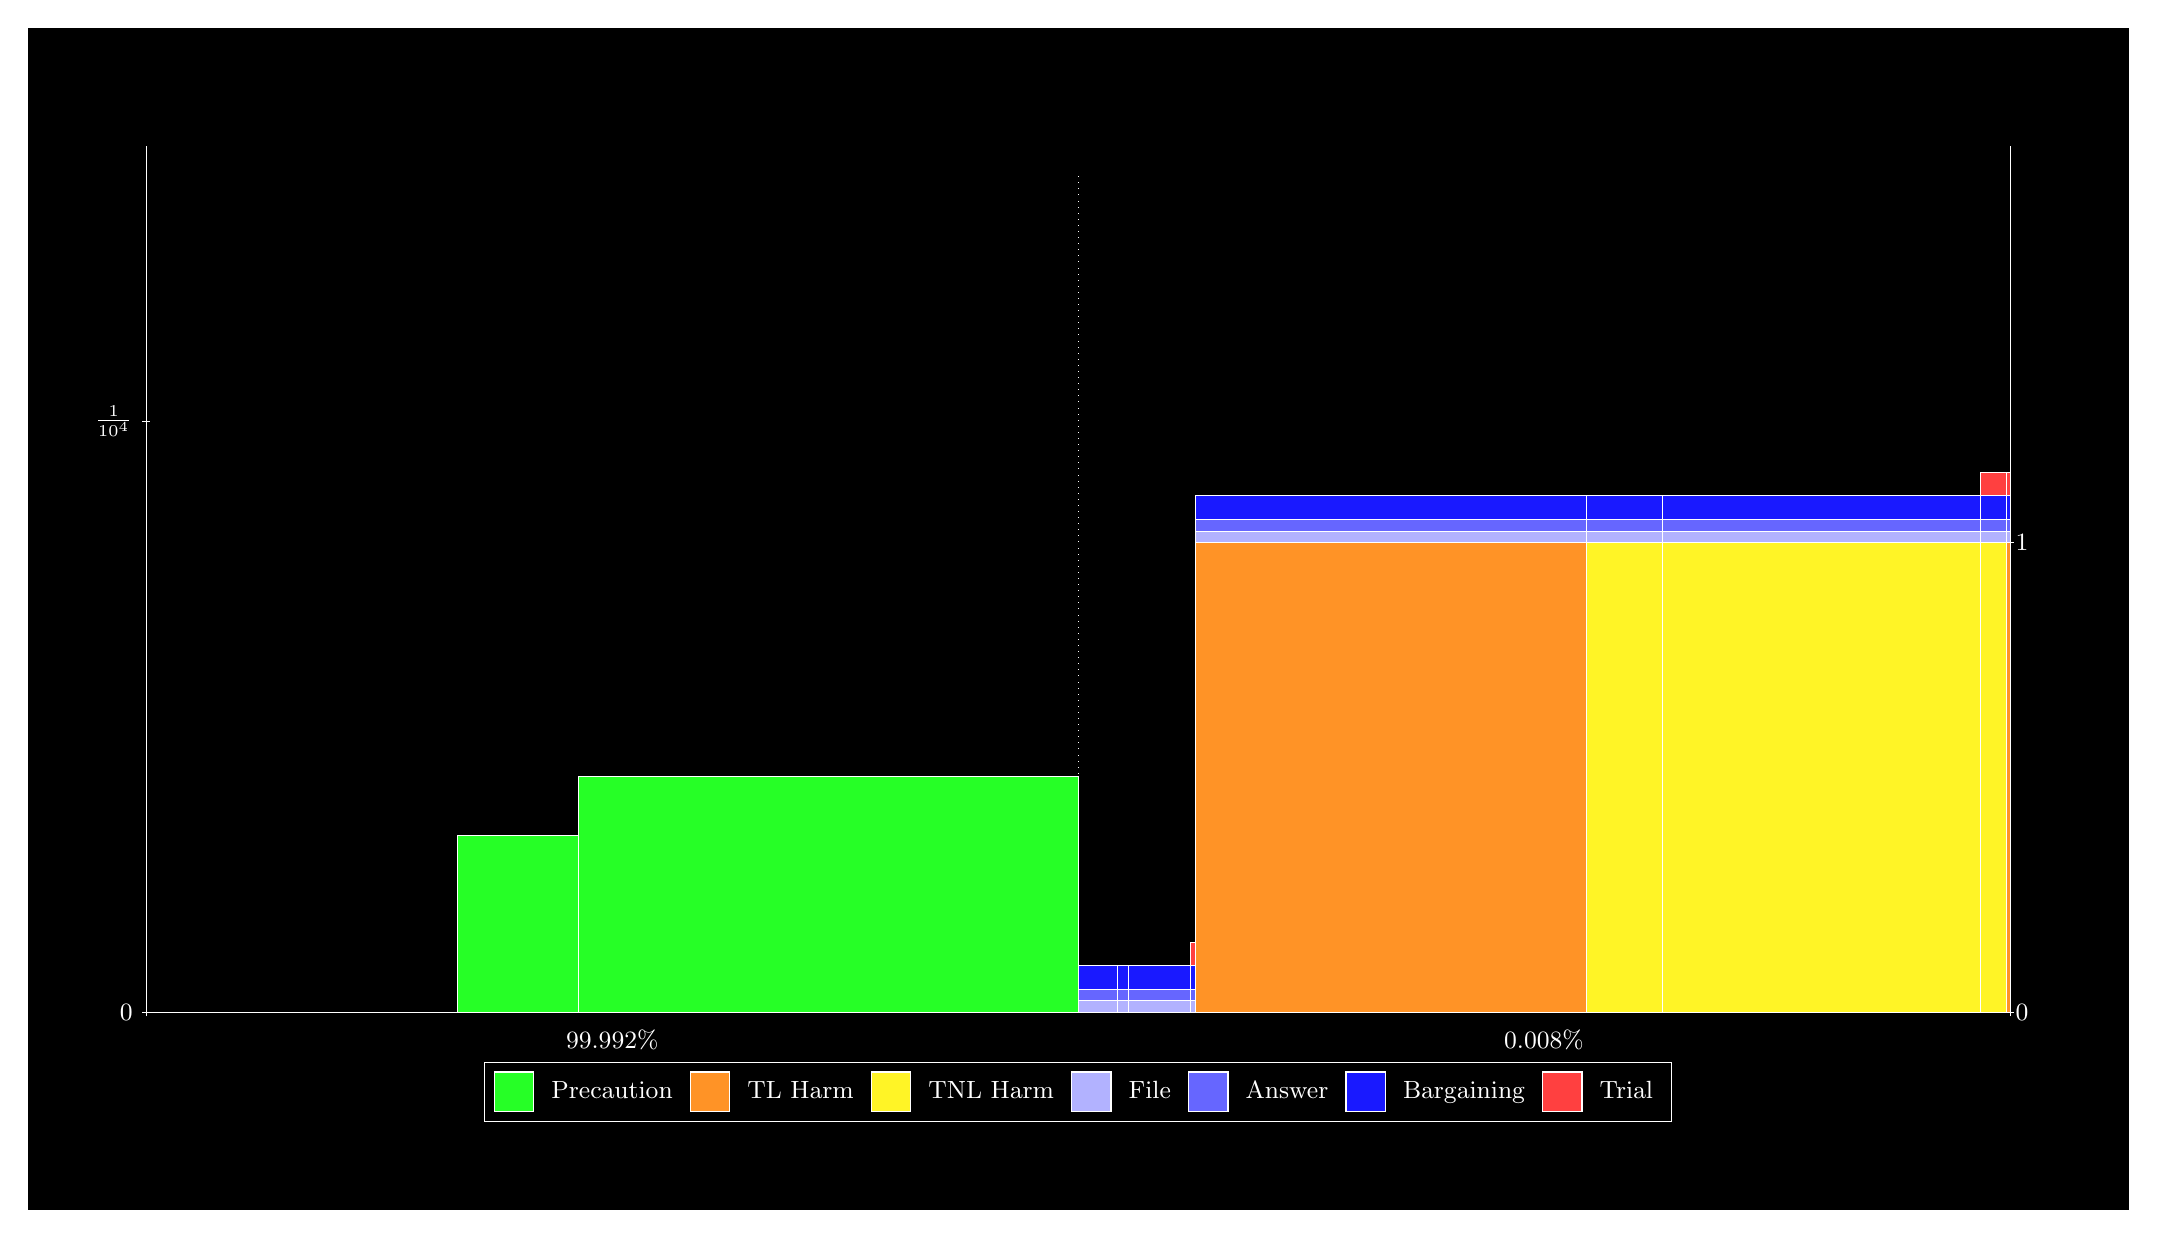
\begin{tikzpicture}
\draw[fill=black] (0,0) rectangle (26.667,15);
\draw[fill=green!85,draw=white,very thin] (5.4443,2.5) rectangle (6.9901,4.7528);
\draw[fill=green!85,draw=white,very thin] (6.9901,2.5) rectangle (13.333,5.5038);
\draw[fill=blue!30,draw=white,very thin] (13.333,2.5) rectangle (13.83,2.6492);
\draw[fill=blue!60,draw=white,very thin] (13.333,2.6492) rectangle (13.83,2.7984);
\draw[fill=blue!90,draw=white,very thin] (13.333,2.7984) rectangle (13.83,3.0968);
\draw[fill=green!85,draw=white,very thin] (13.83,2.5) rectangle (13.965,2.5002);
\draw[fill=blue!30,draw=white,very thin] (13.83,2.5002) rectangle (13.965,2.6494);
\draw[fill=blue!60,draw=white,very thin] (13.83,2.6494) rectangle (13.965,2.7986);
\draw[fill=blue!90,draw=white,very thin] (13.83,2.7986) rectangle (13.965,3.097);
\draw[fill=green!85,draw=white,very thin] (13.965,2.5) rectangle (14.763,2.5002);
\draw[fill=blue!30,draw=white,very thin] (13.965,2.5002) rectangle (14.763,2.6494);
\draw[fill=blue!60,draw=white,very thin] (13.965,2.6494) rectangle (14.763,2.7986);
\draw[fill=blue!90,draw=white,very thin] (13.965,2.7986) rectangle (14.763,3.097);
\draw[fill=green!85,draw=white,very thin] (14.763,2.5) rectangle (14.822,2.5002);
\draw[fill=blue!30,draw=white,very thin] (14.763,2.5002) rectangle (14.822,2.6494);
\draw[fill=blue!60,draw=white,very thin] (14.763,2.6494) rectangle (14.822,2.7986);
\draw[fill=blue!90,draw=white,very thin] (14.763,2.7986) rectangle (14.822,3.097);
\draw[fill=red!75,draw=white,very thin] (14.763,3.097) rectangle (14.822,3.3954);
\draw[fill=orange!85,draw=white,very thin] (14.822,2.5) rectangle (19.786,8.4679);
\draw[fill=blue!30,draw=white,very thin] (14.822,8.4679) rectangle (19.786,8.6171);
\draw[fill=blue!60,draw=white,very thin] (14.822,8.6171) rectangle (19.786,8.7663);
\draw[fill=blue!90,draw=white,very thin] (14.822,8.7663) rectangle (19.786,9.0647);
\draw[fill=green!85,draw=white,very thin] (19.786,2.5) rectangle (20.751,2.5002);
\draw[fill=yellow!85,draw=white,very thin] (19.786,2.5002) rectangle (20.751,8.4681);
\draw[fill=blue!30,draw=white,very thin] (19.786,8.4681) rectangle (20.751,8.6173);
\draw[fill=blue!60,draw=white,very thin] (19.786,8.6173) rectangle (20.751,8.7665);
\draw[fill=blue!90,draw=white,very thin] (19.786,8.7665) rectangle (20.751,9.0649);
\draw[fill=green!85,draw=white,very thin] (20.751,2.5) rectangle (20.754,2.5002);
\draw[fill=orange!85,draw=white,very thin] (20.751,2.5002) rectangle (20.754,8.4681);
\draw[fill=blue!30,draw=white,very thin] (20.751,8.4681) rectangle (20.754,8.6173);
\draw[fill=blue!60,draw=white,very thin] (20.751,8.6173) rectangle (20.754,8.7665);
\draw[fill=blue!90,draw=white,very thin] (20.751,8.7665) rectangle (20.754,9.0649);
\draw[fill=green!85,draw=white,very thin] (20.754,2.5) rectangle (24.788,2.5002);
\draw[fill=yellow!85,draw=white,very thin] (20.754,2.5002) rectangle (24.788,8.4682);
\draw[fill=blue!30,draw=white,very thin] (20.754,8.4682) rectangle (24.788,8.6174);
\draw[fill=blue!60,draw=white,very thin] (20.754,8.6174) rectangle (24.788,8.7666);
\draw[fill=blue!90,draw=white,very thin] (20.754,8.7666) rectangle (24.788,9.065);
\draw[fill=green!85,draw=white,very thin] (24.788,2.5) rectangle (25.124,2.5002);
\draw[fill=yellow!85,draw=white,very thin] (24.788,2.5002) rectangle (25.124,8.4681);
\draw[fill=blue!30,draw=white,very thin] (24.788,8.4681) rectangle (25.124,8.6173);
\draw[fill=blue!60,draw=white,very thin] (24.788,8.6173) rectangle (25.124,8.7665);
\draw[fill=blue!90,draw=white,very thin] (24.788,8.7665) rectangle (25.124,9.0649);
\draw[fill=red!75,draw=white,very thin] (24.788,9.0649) rectangle (25.124,9.3633);
\draw[fill=green!85,draw=white,very thin] (25.124,2.5) rectangle (25.167,2.5002);
\draw[fill=orange!85,draw=white,very thin] (25.124,2.5002) rectangle (25.167,8.4681);
\draw[fill=blue!30,draw=white,very thin] (25.124,8.4681) rectangle (25.167,8.6173);
\draw[fill=blue!60,draw=white,very thin] (25.124,8.6173) rectangle (25.167,8.7665);
\draw[fill=blue!90,draw=white,very thin] (25.124,8.7665) rectangle (25.167,9.0649);
\draw[fill=red!75,draw=white,very thin] (25.124,9.0649) rectangle (25.167,9.3633);
\draw[white,very thin] (1.5,2.5) -- (1.5,13.5);
\draw[white,very thin] (1.45,2.5) -- (1.55,2.5);
\node[font=\small,text=white, anchor=east] at (1.45, 2.5) {0};
\draw[white,very thin] (1.45,10.009) -- (1.55,10.009);
\node[font=\small,text=white, anchor=east] at (1.45, 10.009) {$\frac{1}{10^{4}}$};

\draw[white,dotted,very thin] (13.333,2.83) -- (13.333,13.17);
\draw[white,very thin] (25.167,2.5) -- (25.167,13.5);
\draw[white,very thin] (25.117,2.5) -- (25.217,2.5);
\node[font=\small,text=white, anchor=west] at (25.117, 2.5) {0};
\draw[white,very thin] (25.117,8.4679) -- (25.217,8.4679);
\node[font=\small,text=white, anchor=west] at (25.117, 8.4679) {1};

\draw[white,very thin] (1.5,2.5) -- (25.167,2.5);
\draw[white,very thin] (1.5,2.45) -- (1.5,2.55);
\node[font=\small,text=white, anchor=north] at (1.5, 2.45) {};
\draw[white,very thin] (25.167,2.45) -- (25.167,2.55);
\node[font=\small,text=white, anchor=north] at (25.167, 2.45) {};

\node[font=\small,text=white,anchor=south] at (7.4167, 1.9) {99.992\%};
\node[font=\small,text=white,anchor=south] at (19.25, 1.9) {0.008\%};
\draw (13.3333,2.5) node (B) {};
\begin{scope}[align=center]
\matrix[scale=0.5,draw=white,below=0.5cm of B,nodes={draw},column sep=0.1cm]{
\node[rectangle,draw,minimum width=0.5cm,minimum height=0.5cm,fill=green!85]{}; & \node[draw=none,font=\small,text=white]{Precaution}; &
\node[rectangle,draw,minimum width=0.5cm,minimum height=0.5cm,fill=orange!85]{}; & \node[draw=none,font=\small,text=white]{TL Harm}; &
\node[rectangle,draw,minimum width=0.5cm,minimum height=0.5cm,fill=yellow!85]{}; & \node[draw=none,font=\small,text=white]{TNL Harm}; &
\node[rectangle,draw,minimum width=0.5cm,minimum height=0.5cm,fill=blue!30]{}; & \node[draw=none,font=\small,text=white]{File}; &
\node[rectangle,draw,minimum width=0.5cm,minimum height=0.5cm,fill=blue!60]{}; & \node[draw=none,font=\small,text=white]{Answer}; &
\node[rectangle,draw,minimum width=0.5cm,minimum height=0.5cm,fill=blue!90]{}; & \node[draw=none,font=\small,text=white]{Bargaining}; &
\node[rectangle,draw,minimum width=0.5cm,minimum height=0.5cm,fill=red!75]{}; & \node[draw=none,font=\small,text=white]{Trial}; \\\\
};\end{scope}

\end{tikzpicture}
\end{document}